
\documentclass[12pt]{article}
\pagestyle{empty}
\setlength{\parskip}{0in}
\setlength{\textwidth}{6.8in}
\setlength{\topmargin}{-.5in}
\setlength{\textheight}{9.3in}
\setlength{\parindent}{0in}
\setlength{\oddsidemargin}{-.7cm}
\setlength{\evensidemargin}{-.7cm}

\usepackage{amsmath}
\usepackage{amsthm}
\usepackage{amstext}

\usepackage{graphicx}

\begin{document}

{\bf MAT 105 Final Exam (tan) Fall 2009} \hspace{.4in} {\large Name} \hrulefill

\hspace{.2in}

\begin{center}

\begin{tabular}
{|l|c|c|c|c|c|c|c|c|c|c|c|c|c|c|c|c|} \hline

 Problems & \hspace{5 pt} 1 \hspace{5 pt}  & \hspace{5 pt} 2 \hspace{5 pt} & \hspace{5 pt} 3 \hspace{5 pt} & \hspace{5 pt} 4 \hspace{5 pt}& \hspace{5 pt} 5 \hspace{5 pt} & \hspace{5 pt} 6 \hspace{5 pt} & \hspace{5 pt} 7 \hspace{5 pt}   & \hspace{5 pt} 8 \hspace{5 pt} &  \hspace{5 pt} Total  \hspace{5 pt} & &  \hspace{5 pt} Grade \hspace{5 pt}  \\ \hline
&&&&&&&&&&&\\  
Points &&&&&&&&&&   \hspace{.6in}\% &  \\ 
&&&&&&&&&&& \\  \hline
Out of & 40  & 14 & 28 & 22 & 38 & 17 & 22 & 19 &200 & & \\ \hline

\end {tabular}
 
\end{center}

\hspace{.2in}

\begin{itemize}
\item Relax.  You have done problems like these before. Even if these problems look a bit different, just do what you can. 
\item  If you're not sure of something or if you're stuck, please ask! 
\item You may use your calculator but please show all of your work and write down as many steps as you can.  
\item Some formulas from our book that you might need are on a separate sheet.
\item Don't spend too much time on any one problem.
\item  Do well.  And remember to ask me if you need help.
\end{itemize}

  \vspace{.2in}
 
 \hrulefill
 
\newpage  %%%

\begin{enumerate}
\item Evaluate each of the following expressions.

\begin{enumerate}
\item $29.99 + 2.07(400)=$
\vfill
\item $(34)^2-4(3)(-2)=$
\vfill
\item $3,600(1.02)^{64}=$
\vfill
\item $\displaystyle \frac{-(15)}{2(-9)}=$
\vfill
\item $5^{15}=$
\vfill
\item $(2.3)^{1/5}=$
\vfill
\item $\sqrt{719}=$
\vfill
\item $\displaystyle \frac{\text{log}(34.21)}{\text{log}(1.13)}=$
\vfill
\emph{Write the next answer in normal (expanded) decimal notation.}
\item $4.12 \times 10^{14}=$  


\vfill
\emph{Write the next answer in normal (expanded) decimal notation.}
\item $4.12 \times 10^{-14}=$  


\vfill
\end{enumerate}

\newpage  %%%

\item The 1918 flu season was one of the deadliest in history.  The graph and table show the number of flu deaths in Liverpool, United Kingdom during 1918.

\begin{center}
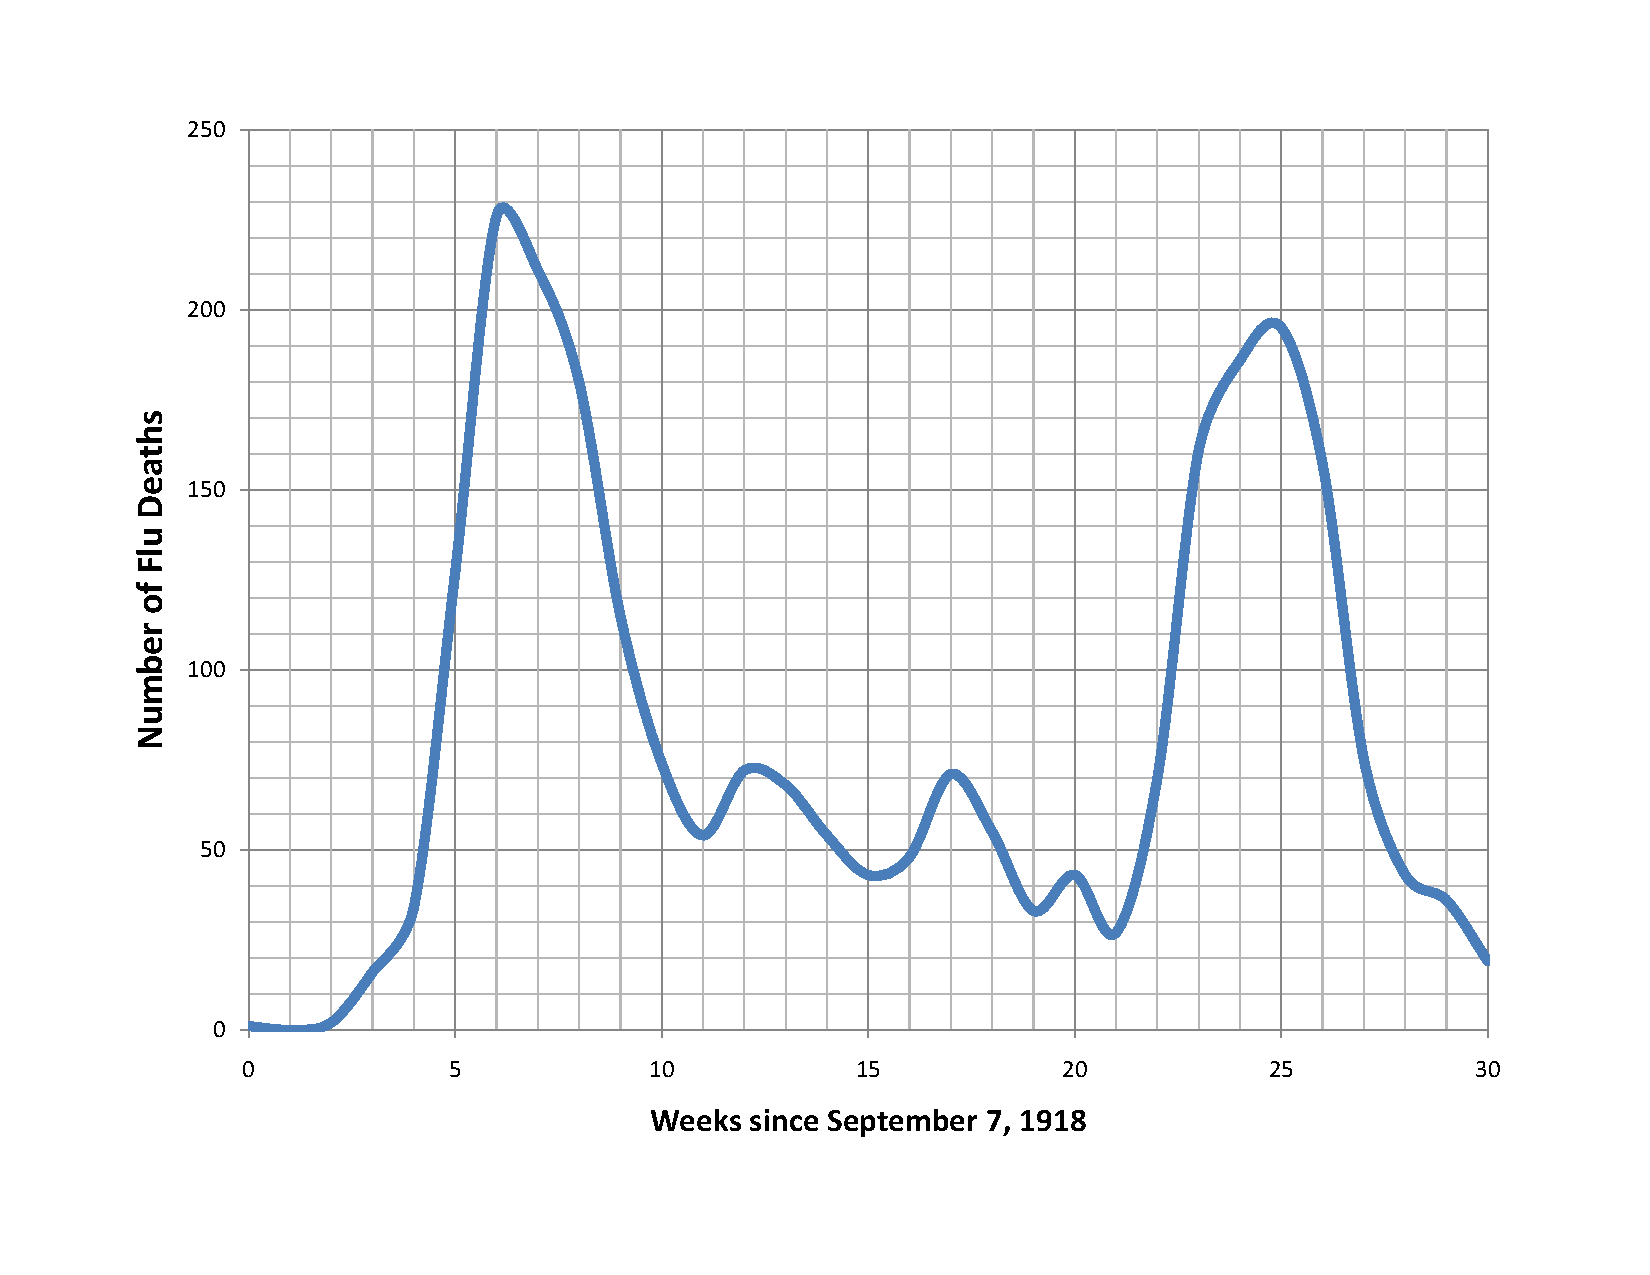
\includegraphics [width = .8\textwidth] {LiverpoolFlu.pdf}
\end{center}

\begin{tabular} {|c|c|c|c|c |c|c|c|c|c |c|c|} \hline
Weeks since Sept. 7, 1918 & 0 & 3 & 6  & 9  & 12  & 15  & 18 & 21  & 24  & 27  & 30 \\ \hline
Number of deaths &1 & 16 & 226 & 115 & 72 & 43 & 55 & 27 & 186 & 75 & 19 \\ \hline
\end{tabular}

\begin{enumerate}
\item How many people died from the flu 9 weeks after September 7?
\vfill
\item In what weeks after September 7 were the number of flu deaths the same as the level at 9 weeks?
\vfill
\item In what week after September 7 was the number of flu deaths the highest and what were the approximate number of deaths?
\vfill
\item Was the number of weekly flu deaths increasing faster 3 weeks after September 7 or 24 weeks after September 7?  Explain. (\emph{Hint: Determine the average rate of change at both of these times.})
\vfill
\end{enumerate}

\newpage %%%

\item My mechanic charges $M$ dollars for $H$ hours of work, as given by the following formula:
$$M = 19.95 + 75.00H$$

\begin{enumerate}
\item Make a table of values showing the charges for 1 hour, 1$\frac{1}{2}$ hours, 2 hours, and 3 hours.
\vfill
\item What does the 19.95 represent and what are its units?
\vfill
\item What does the 75.00 represent and what are its units?
\vfill
\item If the bill for my last visit to the mechanic was $\$638.70$, how much time did he work?

\emph{Set up and solve an equation to answer the question.  If you can't solve it, then you may estimate the answer to two decimal places for possible partial credit.}
\vfill
\vfill
\vfill
\item Convert your answer to the nearest minute.
\vfill
She worked for \hrulefill hours, \hrulefill minutes. \hspace{3in}.
\end{enumerate}

\newpage %%%
\item The timing of the sunrise depends on the latitude (how far North of South of the equator one is) and the time of year.  In Minneapolis, the sunrise occurred at 4:30 AM on July 1.  The time of the sunrise is expected to occur 0.74 minutes later each day.  In Panama City, Florida, the sunrise occurred at 4:45 AM on July 1 and is expected to occur 0.49 minutes later each day.  (Note: do not worry about Daylight Savings Time.) If we let $S$ represent the time of the sunrise (in minutes since 4:00 AM) for $D$ days after July 1, then the equations are:

\vspace{.1in}

\begin{center}
\begin{tabular} {ll} 
Minneapolis: &$S=30+0.74D$ \\
Panama City: & $S=45+0.49D$ \\
\end{tabular}
\end{center}

The table shows sunset times for the two cities:

\begin{center}
\begin{tabular} {|l|r|r|r|r|} \hline
$D$ & 0 & 10 & 30 & 70 \\ \hline
$S$ (Minneapolis) & 30 &  37.4 & 52.2 & 81.8  \\ \hline
$S$ (Panama City) & 45 & 49.9 & 59.7 & 79.3 \\ \hline
\end{tabular}
\end{center}


\begin{enumerate}

\item Which city has a later sunrise on July 25 (i.e. after 25 days)?  \emph{Justify your answer.}
\vfill
\item Draw a graph illustrating both equations.
\vspace{.1in}
\begin{center}
\scalebox {.8} {
\includegraphics [width = 6in] {../GraphPaper}}
\end{center}
\vfill
\emph{The problem continues on the next page ...}
\pagebreak
\item Set up and solve an equation to find when the two cities will have the sunset at the same time. Report your answer to the nearest day.

\emph{Just approximating the answer will get almost no partial credit.}

\vfill
\vfill
\vfill
\end{enumerate}

\newpage %%%

\item Joy jumped from a rock into an abandoned mining pit filled with water. The rock ledge was 10 meters above the ground.  Her height above the water, $H$ meters, after $T$ seconds is given by the formula: $$H = 10 + 3.2T - 4.88T^2$$

\begin{enumerate}
\item Complete the following table of values.

\emph{Please report your answers to the first two decimal places.}

\begin{center}
\begin{tabular} {|l|c|c|c|c|c|c|} \hline
$T$ & 0 & 0.5 & 0.8 & 1.0 & 1.6 & 2.0 \\ \hline
&&&&&& \\
$H$ & \hspace{.7in} & \hspace{.7in}  & \hspace{.7in}  & \hspace{.7in}  & \hspace{.7in}  & \hspace{.7in}  \\
&&&&&& \\ \hline
\end{tabular}
\end{center}

\item How high up in the air does Joy get?

\emph{Find the answer to two decimal places using whatever method you prefer.}
\vfill
\vfill

\item Convert your answer to the nearest foot.  \emph{Use 1 meter = 3.28 feet.}
\vfill

\hspace{-.5in} \emph{The problem continues on the next page.}

\newpage %%%

\item Draw a graph illustrating the dependence.

\vspace{.1in}
\begin{center}
\scalebox {.8} {
\includegraphics [width = 6in] {../GraphPaper}}
\end{center}
\vspace{.1in}

\item When does Joy hit the water?

\emph{Find the answer to two decimal places using whatever method you prefer.}

\vfill
\end{enumerate}

\newpage %%%
%%% http://www.energywatchgroup.org/fileadmin/global/pdf/2009-01_Wind_Power_Report.pdf

\item A recent summit in Copenhagen is focusing on climate change and its impacts.  Increasing carbon dioxide emissions are a cause of concern because of their linkages to climate change.  In 1959 (when modern instruments could first measure carbon dioxide concentrations), the average concentration in the Northern Hemisphere was 316 parts per million (ppm) CO$_{2}$.  That is to say, there were 316 CO$_{2}$ molecules for every million molecules of air.  In 1990, the concentration of CO$_{2}$ was 354 ppm CO$_{2}$.  Assuming this increase is exponential, from 1990 to 2008 the CO$_{2}$ concentration grew at a rate of 0.27\% per year.  That is, the CO$_{2}$ concentration $C$ (in ppm) $Y$ years after 1959 is given by the equation:

$$C=316(1.0027)^Y$$

\begin{enumerate}
\item According to this equation, what will the CO$_{2}$ concentration be in 2010?
\vfill
\item If the value continues to increase, in what year will the CO$_{2}$ concentration be over 400 parts per million CO$_{2}$?

\emph{Set up and solve an equation to answer the question.  If you can't solve it, then you may estimate the answer for possible partial credit.}
\vfill
\vfill
\vfill
\end{enumerate}

\newpage %%%

\item I had to rent a sod roller from Home Depot when I laid sod in my back yard last summer.    The table below lists the rental charges for the roller.  They charge an initial fee plus an hourly rate.

\begin{center}
\begin{tabular} {|r|r|r|r|r|r|r|} \hline
Hours & 1 & 2 & 3 & 4 & 5 & 10 \\ \hline
Cost & \$15.90 & \$21.15 & \$26.40 & \$31.65 & \$36.90 & \$63.15 \\ \hline
\end{tabular}
\end{center}

\begin{enumerate}
\item Name the variables including units.
\vfill
\item What does the Home Depot charge per hour for the tool rental?
\vfill
\item What is the initial fee?
\vfill
\item Write an equation describing the cost of renting a sod roller.
\vfill
\end{enumerate}

\newpage %%%
%%% http://en.wikipedia.org/wiki/List_of_newspapers_in_the_United_States_by_circulation
%%% http://www.infoplease.com/ipea/A0004420.html
\item Newspaper subscriptions have dropped as more people use the internet for news.  In 2006, the New York Times had 1,683,855 subscribers.  Today in 2009 (3 years later), only 927,851 people subscribe to the paper. You can assume that the decline is exponential.

\begin{enumerate}
\item By what percentage has the number of subscribers dropped each year?
\vfill
\item If this trend continues, what will the number of subscribers be in 2012 (i.e.\ after 6 years from 2006)?
\vfill
\end{enumerate}



\end{enumerate}

\end{document}

